\documentclass[t,mathserif]{beamer}

% no paragraph indenting
\usepackage{parskip}

% use the helvetic font for sans-serif fonts
%\usepackage{helvetic}

\usepackage[english]{babel}
\usepackage{csquotes}

\usepackage{subfigure}

\usepackage{textpos}

\usepackage[nolist]{acronym}

%-------------------------------------------------------------------------------
% math

% advanced mathematical expressions
\usepackage{amsmath}

% math fonts (i.e. \mathbb{R} for the real set symbol)
\usepackage{amsfonts}

% relation symbols
\usepackage{amssymb}

\usepackage{amsthm}

% allow math expressions as latex command parameters
% (i.e. \setlength{\textwidth}{\textwidth - 5cm})
\usepackage{calc}
\usepackage{wasysym}

\usepackage{mathtools}


%-------------------------------------------------------------------------------
% graphics

\usepackage{graphicx}   % eXtended GRAPHICs package
\DeclareGraphicsExtensions{.pdf,.png,.jpg}
\graphicspath{ {pics/} }


%-------------------------------------------------------------------------------
% colors

% imports definecolor (see grfguide) and named colors
%\usepackage[usenames]{color}
\definecolor{darkblue}{rgb}{0, 0, 0.5}
\definecolor{darkgreen}{rgb}{0, 0.5, 0}
\definecolor{shaded}{gray}{.6}

%-------------------------------------------------------------------------------
% multimedia

\usepackage{multimedia}


%-------------------------------------------------------------------------------
% table extensions
\usepackage{array}
\usepackage{multirow}
\usepackage{colortbl}
%\setlength{\extrarowheight}{1mm}
\usepackage{booktabs}


%-------------------------------------------------------------------------------
% source code listings

%\usepackage{listings}
%\lstset{numbers=left, numberstyle=\tiny, numbersep=5pt, tabsize=4, extendedchars=true}
%\lstloadlanguages{}
\usepackage[english,ruled,lined,linesnumbered, nofillcomment]{algorithm2e}
%\dontprintsemicolon
\usepackage{listings}
%\usepackage[usenames,dvipsnames]{xcolor}
\usepackage{caption}
\DeclareCaptionFormat{myformat}{\hrulefill\\#1#2#3}
\captionsetup[lstlisting]{singlelinecheck=off,format=myformat}
\captionsetup[table]{font=small}
% the frame of the listings environment extends outside of the actual space reserved for the listings environment, hence the extra margin parameters become necessary
\newlength{\lstvertmargin}
\setlength{\lstvertmargin}{\medskipamount+2ex}
\lstset{frame=single,framesep=2ex,xleftmargin=2ex,xrightmargin=2ex,aboveskip=\lstvertmargin,belowskip=\lstvertmargin,language=c++,basicstyle=\small\usefont{T1}{pcr}{m}{n},extendedchars=true,tabsize=3}

%-------------------------------------------------------------------------------
% custom commands

\newcommand{\mat}[1]{{\bf #1}}
\newcommand{\R}{\mathbb{R}}
\newcommand{\reffig}[1]{\ref{#1}}
%ifdef RELEASE
% % \newcommand{\todo}[1]{}
%else
\newcommand{\todo}[1]{\textcolor{red}{TODO}~#1}
%endif
\newcommand{\abs}[1]{\lvert#1\rvert}
\newcommand{\norm}[1]{\lVert#1\rVert}
\newcommand{\jac}[2]{\partial #1#2}

\newcommand{\vlinecenter}[1]{\raisebox{(\ht\strutbox - \totalheight)*\real{0.5}}{#1}}
\newcommand{\spanop}{\operatornamewithlimits{span}}
        


%-------------------------------------------------------------------------------
% about document

\setbeamercolor{itemize items}{fg=black}
\usepackage{fancybox}

\setbeamercolor{block title}{bg=white!90!black}
\setbeamerfont {block title}{series=\bfseries}
\setbeamercolor{block body}{bg=white!90!black}
% \setbeamercolor{block title alerted}{bg=white!90!black}
% \setbeamerfont {block title alerted}{series=\bfseries}
% \setbeamercolor{block body alerted}{bg=white!90!black}
% \setbeamercolor{block title example}{bg=white!90!black}
% \setbeamerfont {block title example}{series=\bfseries}
\setbeamercolor{block body example}{bg=white!90!black}


%-------------------------------------------------------------------------------
% about document
\usepackage{lssbeamer_FAU}
\author{Sam Nees, Paul Mildenberger, Siegfried Sch\"ofer}
\institute[LSS]{Chair for System Simulation}
\title[NuSiF]{Project Chemical Species Transport}
\date[3/2/2014]{February 3rd 2014}

\usepackage{url}

\setbeamertemplate{caption}[numbered]
\setbeamertemplate{caption}{\insertcaption}

\begin{document}

\lstset{
backgroundcolor=\color{white},
basicstyle=\Large,
breakatwhitespace=true,
breaklines=true,
captionpos=t,
commentstyle=\color{green!60!black},
escapeinside={\%*}{*)},
extendedchars=true,
keywordstyle=\color{blue!60!black},
language=C++,
morekeywords={std,vector,string},
frame=tb,
numbers=left,
numbersep=10pt,
numberstyle=\footnotesize\color{gray},
rulecolor=\color{black},
showspaces=false,
showstringspaces=false,
showtabs=false,
stepnumber=1,
stringstyle=\color{red!60!black},
tabsize=4,
xleftmargin=\parindent,
numberblanklines=true,
breakautoindent=true,
}

%**************************************************************************************************
% TITLE PAGE AND OUTLINE
%**************************************************************************************************

%**************************************************************************************************
\begin{frame}[plain,c]
   \titlepage
\end{frame}


%**************************************************************************************************
\begin{frame}[squeeze]
   \frametitle{Outline}\tableofcontents
\end{frame}


%**************************************************************************************************

\section{Discretization of the concentration convection-diffusion equation}
\subsection{Fundamental equation}
\begin{frame}[allowframebreaks]{Fundamental equation}
	\begin{equation}
\frac{\partial c}{\partial t} + \vec{u} \cdot \nabla c = \lambda \Delta c + Q(t,x,y,\vec{u},c)
\end{equation}
\begin{itemize}
	\item $\lambda$ diffusion coefficient
	\item $Q$ source term (location, time, velocity, concentration), multi-species-systems are modeled here
	\item the chemical processes under consideration have no effect on the density and hence produce no buoyancy forces $\Rightarrow$ no coupling with the momentum equations
	\item convective transport: $\vec{u} \cdot \nabla c$
	\item diffusive spreading: $\lambda \Delta c$
	\item time step control necessary
    \item for very stiff equations, implicit procedures might be necessary, we do an explicit time stepping
\end{itemize}
\end{frame}

\subsection{Boundary conditions}
\begin{frame}{Boundary conditions}
\begin{itemize}
	\item Dirichlet BC when injecting concentration
	\item Neumann BC for impermeable walls
\end{itemize}
\end{frame}

\subsection{Discretization}
\begin{frame}[allowframebreaks]{Discretization}
\begin{equation}
\left \lbrack \frac{\partial c}{\partial t} \right \rbrack_{ij}^{n+1} + \left
\lbrack \frac{\partial uc}{\partial x} \right \rbrack_{ij} + \left \lbrack
\frac{\partial vc}{\partial y} \right \rbrack_{ij} = \lambda \left \lbrack
\frac{\partial^2 c}{\partial x^2} + \frac{\partial^2 c}{\partial y^2} \right \rbrack_{ij} + Q_{ij}
\end{equation}
\begin{equation}
\left \lbrack \frac{\partial c}{\partial t} \right \rbrack_{ij}^{n+1} =
\frac{1}{dt} \left (c_{ij}^{n+1} - c_{ij}^n \right )
\end{equation}
\begin{equation}
\begin{aligned}
\left \lbrack \frac{\partial uc}{\partial x} \right \rbrack_{ij} =
\frac{1}{dx} \left (u_{ij} \frac{c_{ij}+c_{i+1,j}}{2} - u_{i-1,j}
\frac{c_{i-1,j}+c_{ij}}{2} \right) + \\
\frac{\gamma}{dx} \left (|u_{ij}| \frac{c_{ij}-c_{i+1,j}}{2} - |u_{i-1,j}|
\frac{c_{i-1,j}-c_{ij}}{2} \right)
\end{aligned}
\end{equation}
\pagebreak
\begin{equation}
\begin{aligned}
\left \lbrack \frac{\partial vc}{\partial y} \right \rbrack_{ij} =
\frac{1}{dy} \left (v_{ij} \frac{c_{ij}+c_{i,j+1}}{2} - v_{i,j-1}
\frac{c_{i,j-1}+c_{ij}}{2} \right) + \\
\frac{\gamma}{dy} \left (|v_{ij}| \frac{c_{ij}-c_{i,j+1}}{2} - |v_{i,j-1}|
\frac{c_{i,j-1}-c_{ij}}{2} \right)
\end{aligned}
\end{equation}
\begin{equation}
\left \lbrack \frac{\partial^2 c}{\partial x^2} \right \rbrack_{ij} =
\frac{c_{i+1,j} -2 c_{ij} + c_{i-1,j}}{(dx)^2}
\end{equation}
\begin{equation}
\left \lbrack \frac{\partial^2 c}{\partial y^2} \right \rbrack_{ij} =
\frac{c_{i,j+1} -2 c_{ij} + c_{i,j-1}}{(dy)^2}
\end{equation}

\begin{itemize}
	\item concentration $c$ lies on the center of the staggered grid cell
	\item standard central differences of the Laplacian
	\item add timestep control
\end{itemize}
\end{frame}

\subsection{Timestep Control}
\begin{frame}{Timestep Control}
	\begin{equation}
			dt < \frac{1}{2 \lambda_i} \left ( \frac{1}{(dx)^2} +
			\frac{1}{(dy)^2} \right ) ^{-1}
	\end{equation}
	\begin{itemize}
		\item has to be added for every new species
		\item depends on the diffusion constant
	\end{itemize}
\end{frame}

\subsection{Implementation}
\begin{frame}[allowframebreaks]{Implementation}
\begin{itemize}
	\item array of Arrays for multiple concentrations
	\item array of reals for the lambdas
	\item the reaction term $Q$ is also stored in Arrays
	\item extended parameter reader
	\item extended initialization
\end{itemize}
\framebreak
\textbf{Main loop:}
\begin{itemize}
	\item determineNextDT: added support for the concentration convection diffusion equation
    \item refreshBoundaries: Dirichlet and Neumann BC according to input for every species (e.g. iterate over all Arrays)
    \item computeFG: no change
    \item composeRHS: no change
    \item calculateConcentrations: explicit concentration update
    \item updateVelocities: no change
    \item vtk: support for multiple concentrations
\end{itemize}
\end{frame}

\subsection{Results}
\begin{frame}[allowframebreaks]{Results}
\begin{itemize}
	\item two species come together at an obstacle and create a new one
	\item one species is coming from west and east
	\item the other from the south
\end{itemize}
\framebreak
\begin{center}
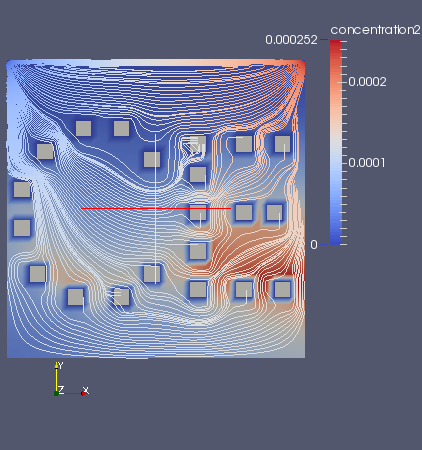
\includegraphics[width=0.6\textwidth]{result1.png}
\end{center}
\end{frame}

\end{document}
